% !TeX root = ../main.tex

\addchap{Appendix} \label{chapter:appendix}

\refstepcounter{chapter} 
\section{Images}

\begin{figure}[h!tb]
\centering
\begin{subfigure}{1.0\textwidth}
  \centering
  \adjincludegraphics[width=1.0\linewidth,trim={0 0 0 0},clip]{figures/ds/ucf_train_full.png}
  \caption{Training set}
  \label{fig:ucf_train_full}
  \vspace{.1cm}
\end{subfigure}
\caption[UCF-101 Full Image Samples]{Randomly chosen and rescaled clip samples of size $160 \times 120$ from the UCF-101 dataset. There is only a very small portion of motion to see between one frame to the next, because the videos have a frame rate of \num{25} FPS.\\
\textit{(continues on next page)}}
\label{fig:ucf_full}
\end{figure}



\begin{figure}[h!tb]
\ContinuedFloat % continue from previous page
\centering
\begin{subfigure}{1.0\textwidth}
  \centering
  \adjincludegraphics[width=1.0\linewidth,trim={0 0 0 0},clip]{figures/ds/ucf_valid_full.png}
  \caption{Validation set}
  \label{fig:ucf_valid_full}
  \vspace{.1cm}
\end{subfigure}
\begin{subfigure}{1.0\textwidth}
  \centering
  \adjincludegraphics[width=1.0\linewidth,trim={0 0 0 0},clip]{figures/ds/ucf_test_full.png}
  \caption{Test set}
  \label{fig:ucf_test_full}
\end{subfigure}
\caption*{}
\end{figure}







\begin{figure}[h!tb]
\centering
\begin{subfigure}{1.0\textwidth}
  \centering
  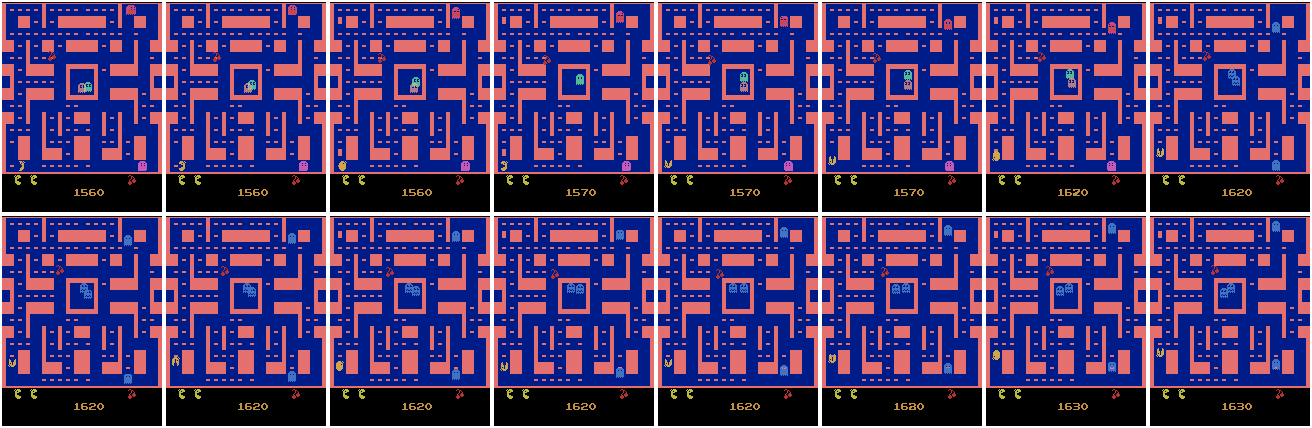
\includegraphics[width=1.0\linewidth]{figures/ds/pac_train_full.png}
  \caption{Training set}
  \label{fig:pac_train_full}
  \vspace{.1cm}
\end{subfigure}
\begin{subfigure}{1.0\textwidth}
  \centering
  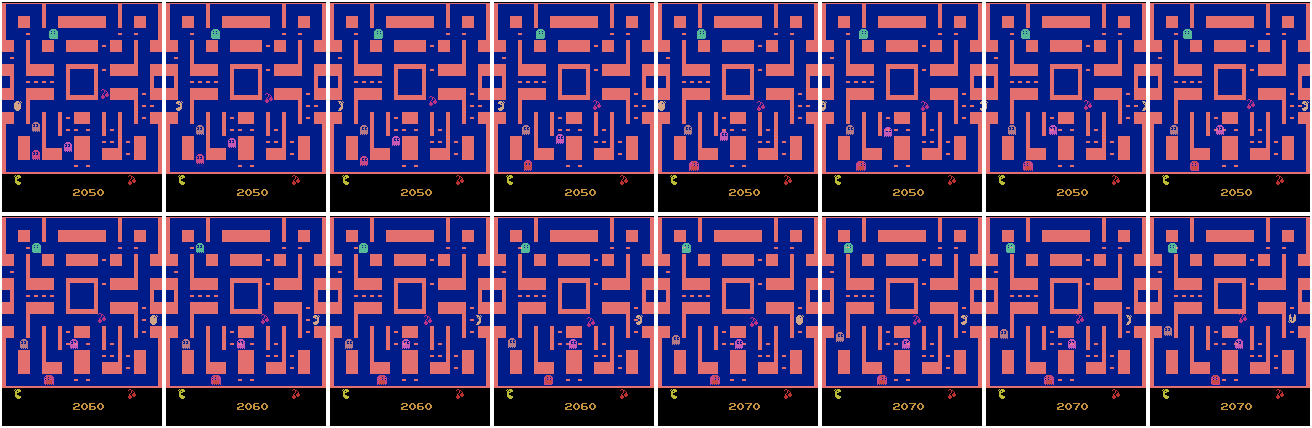
\includegraphics[width=1.0\linewidth]{figures/ds/pac_valid_full.png}
  \caption{Validation set}
  \label{fig:pac_valid_full}
  \vspace{.1cm}
\end{subfigure}
\begin{subfigure}{1.0\textwidth}
  \centering
  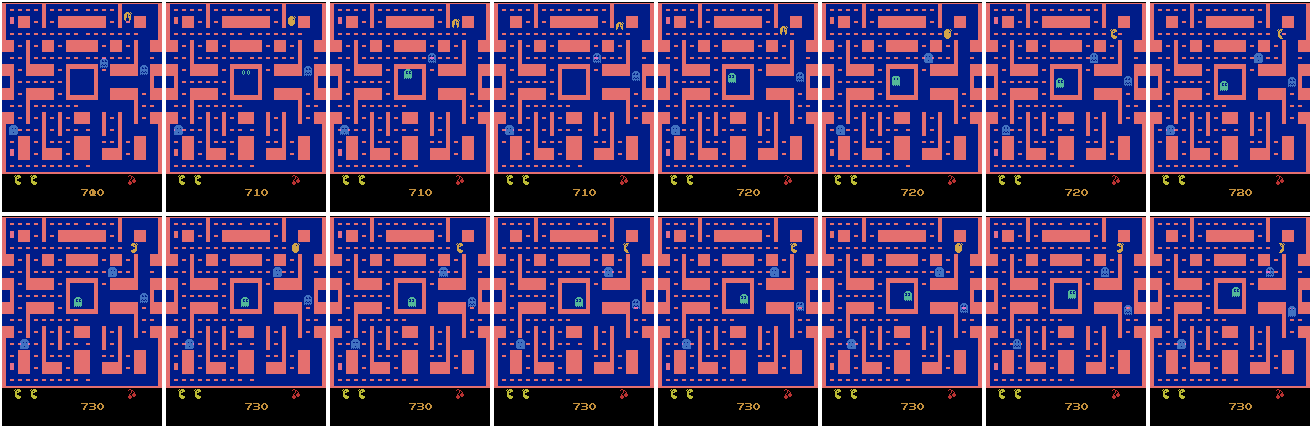
\includegraphics[width=1.0\linewidth]{figures/ds/pac_test_full.png}
  \caption{Test set}
  \label{fig:pac_test_full}
\end{subfigure}
\caption[MsPacman Full Image Samples]{Exemplary sequences of game recordings from MsPacman dataset that have been samples randomly from the different splits. Each shown clip has a length of \num{16} frames of size $160 \times 210$.}
\label{fig:pacman_full}
\end{figure}



\clearpage
\section{Code Listings}

\begin{figure}[h!tb]
  \lstinputlisting[language=PythonEx]{code/model.py}
  \caption[Code: Convolutional Autoencoder]{An example implementation of a convolutional autoencoder model that has an encoder and decoder with two layers each.}\label{code:model}
\end{figure}





